\documentclass{standalone}

%%%%%%%%%%%%%%%%%%%%%%%%%%%%%%%%%%%%%%
% Packages ---------------------------------------------------------
%%%%%%%%%%%%%%%%%%%%%%%%%%%%%%%%%%%%%%
\usepackage[version=4]{mhchem}				 % chemical reactions environment
\usepackage{tikz}										 % Tikz package
\usetikzlibrary{arrows.meta}						% Pacakge for Arrows
\usepackage{amssymb} 								% Package for empty set

%%%%%%%%%%%%%%%%%%%%%%%%%%%%%%%%%%%%%%
% Commands  ------------------------------------------------------
%%%%%%%%%%%%%%%%%%%%%%%%%%%%%%%%%%%%%%
\renewcommand{\familydefault}{\sfdefault}        	% Change Font
\let\emptyset\varnothing

%%%%%%%%%%%%%%%%%%%%%%%%%%%%%%%%%%%%%%
% Commands  ------------------------------------------------------
%%%%%%%%%%%%%%%%%%%%%%%%%%%%%%%%%%%%%% 
\newcommand{\species}[1]{{\bf\ce{#1}}}
\newcommand{\UP}[1]{\makebox[0pt]{\smash{\raisebox{1em}{\normalsize #1}}}}
\newcommand{\RT}[1]{\makebox[0pt]{\hspace{5em}$#1$}}

%%%%%%%%%%%%%%%%%%%%%%%%%%%%%%%%%%%%%%
% Colors ------------------------------------------------------------
%%%%%%%%%%%%%%%%%%%%%%%%%%%%%%%%%%%%%%
\definecolor{Repressor}{RGB}{228,26,28}
\definecolor{Activator}{RGB}{77,175,74}
\definecolor{NAR}{RGB}{150,150, 150}

%%%%%%%%%%%%%%%%%%%%%%%%%%%%%%%%%%%%%%
% Elements  --------------------------------------------------------
%%%%%%%%%%%%%%%%%%%%%%%%%%%%%%%%%%%%%%
\newcommand{\Species}[5]{ % Inputs: coordinates, scale, color, name, textcolor
	\begin{scope}[shift = {(#1)}, scale = #2]	
		\filldraw[fill=#3, draw=black, thick] (0,0) circle (0.5cm);
		%		\filldraw[fill=#3, draw=black, thick, blur shadow ={shadow opacity=80, shadow blur steps=50}] (0,0) circle (0.5cm);
		\node[anchor = center, #5] at (0,0) {\Large #4};
	\end{scope}
}

\newcommand{\Dimer}[6]{ % Inputs: coordinates, scale, color, name, textcolor, rotation
	\begin{scope}[shift = {(#1)}, scale = #2, rotate = #6]	
		\filldraw[fill=#3, draw=black, thick] (0.3,0) circle (0.5cm);
		\filldraw[fill=#3, draw=black, thick] (-0.3,0) circle (0.5cm);
		\filldraw[fill=#3, draw = #3] (-0.3,-0.38) rectangle (0.3,0.28);
		\node[anchor = center, #5] at (0,0) {\Large #4};
	\end{scope}
}

\newcommand{\SingleCharge}[4]{ % Inputs: coordinates, scale, rotation, Charge
	\begin{scope}[shift = {(#1)}, scale = #2, rotate = #3]	
		\filldraw[fill=yellow!50, draw=black, ultra thick, rounded corners = 0.1] (-0.2,-0.2) rectangle(0.2,0.2);
		\node [anchor = center] at (0,0) {\Large #4};
	\end{scope}
}

\newcommand{\DoubleCharge}[5]{ % Inputs: coordinates, scale, rotation, Charge1, Charge2
	\begin{scope}[shift = {(#1)}, scale = #2, rotate = #3]	
		\filldraw[fill=yellow!50, draw=black, ultra thick, rounded corners = 0.1] (-0.4,-0.2) rectangle(0,0.2);
		\filldraw[fill=yellow!50, draw=black, ultra thick, rounded corners = 0.1] (0,-0.2) rectangle(0.4,0.2);
		\node [anchor = center] at (-0.2,0) {\Large #4};
		\node [anchor = center] at (0.2,0) {\Large #5};
	\end{scope}
}
%%%%%%%%%%%%%%%%%%%%%%%%%%%%%%%%%%%%%%
% Documents Begins Here ------------------------------------------
%%%%%%%%%%%%%%%%%%%%%%%%%%%%%%%%%%%%%%
\begin{document}
	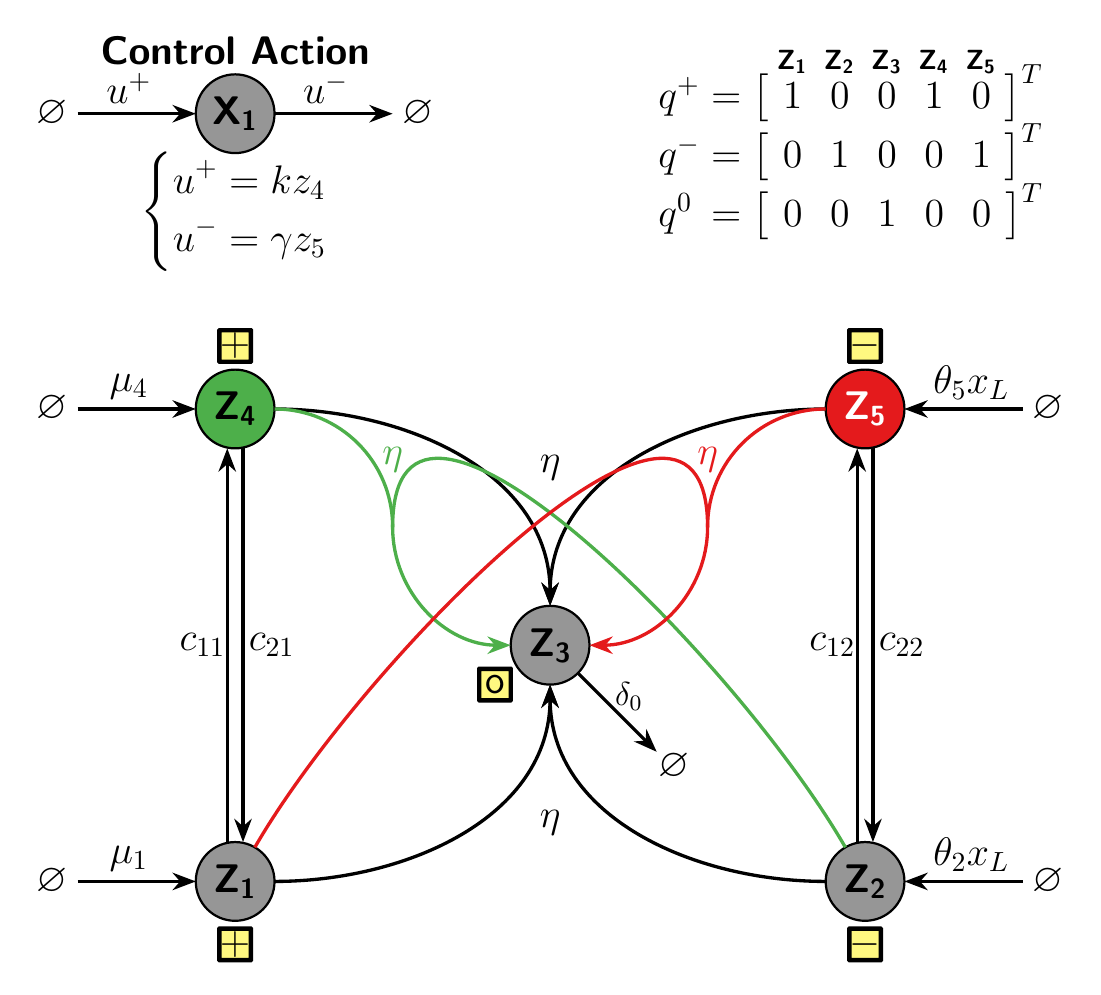
\begin{tikzpicture} 
		%\draw [step=1, very thin, orange] (-8,-1) grid (8,10); 
		%%%%%%%%%%%%%%%%%%%%%%%%%%%%%%%%%%%%%%
		% Blocks -----------------------------------------------------------
		%%%%%%%%%%%%%%%%%%%%%%%%%%%%%%%%%%%%%%
		%\filldraw [IColor!15, rounded corners = 10] (-6.7,-3.2) rectangle (9,0.6);
		
		%%%%%%%%%%%%%%%%%%%%%%%%%%%%%%%%%%%%%%
		% Species -----------------------------------------------------------
		%%%%%%%%%%%%%%%%%%%%%%%%%%%%%%%%%%%%%%
		\Species{(-4,0)}{1}{NAR}{\species{Z_1}}{black};
		\Species{(4,0)}{1}{NAR}{\species{Z_2}}{black};
		\Species{(0,3)}{1}{NAR}{\species{Z_3}}{black};
		\Species{(-4,6)}{1}{Activator}{\species{Z_4}}{black}{0};
		\Species{(4,6)}{1}{Repressor}{\species{Z_5}}{white}{0};
		\Species{(-4,9.75)}{1}{NAR}{\species{X_1}}{black};
		
		%%%%%%%%%%%%%%%%%%%%%%%%%%%%%%%%%%%%%%
		% Charges ----------------------------------------------------------
		%%%%%%%%%%%%%%%%%%%%%%%%%%%%%%%%%%%%%%
		\SingleCharge{(-4,-0.8)}{1}{0}{$+$}; % Z1
		\SingleCharge{(4,-0.8)}{1}{0}{$-$}; % Z2
		\SingleCharge{(-0.7,2.5)}{1}{0}{o}; % Z3
		\SingleCharge{(-4,6.8)}{1}{0}{$+$}; % Z4
		\SingleCharge{(4,6.8)}{1}{0}{$-$}; % Z5
		
		%%%%%%%%%%%%%%%%%%%%%%%%%%%%%%%%%%%%%%
		% Arrows -----------------------------------------------------------
		%%%%%%%%%%%%%%%%%%%%%%%%%%%%%%%%%%%%%%
		\draw [->, -Stealth, very thick] (-6,0) -- (-4.5,0); % Production of Z1
		\draw [->, -Stealth, very thick] (6,0) -- (4.5,0); % Production of Z2
		\draw [->, -Stealth, very thick] (-6,6) -- (-4.5,6); % Production of Z4
		\draw [->, -Stealth, very thick] (6,6) -- (4.5,6); % Production of Z5
		\draw [->, -Stealth, very thick] (-3.5, 0) to [out = 0, in = -90] (0,2.5); % Sequestration of Z1 with Z2
		\draw [->, -Stealth, very thick] (3.5, 0) to [out = 180, in = -90] (0,2.5); % Sequestration of Z2 with Z1
		\draw [->, -Stealth, very thick] (-3.5, 6) to [out = 0, in = 90] (0,3.5); % Sequestration of Z4 with Z5
		\draw [->, -Stealth, very thick] (3.5, 6) to [out = 180, in = 90] (0,3.5); % Sequestration of Z5 with Z4
		
		\draw [->, -Stealth, very thick] (-4.1,0.5) -- (-4.1,5.5); % Association of Z1
		\draw [->, -Stealth, very thick] (-3.9,5.5) -- (-3.9,0.5); % Dissociation of Z4
		\draw [->, -Stealth, very thick] (4.1,5.5) -- (4.1,0.5); % Dissociation of Z2
		\draw [->, -Stealth, very thick] (3.9,0.5) -- (3.9,5.5); % Association of Z5
		
		\draw [very thick, Activator] (4-0.5*cos{60}, 0.5*sin{60}) to [out = 90+30, in = 90] (-2,4.5); % Sequestration of Z2 with Z4
		\draw [very thick, Activator] (-4+0.5,6) to [out = 0, in = 90 ] (-2,4.5); % Sequestration of Z4 with Z2
		\draw [->, -Stealth, very thick, Activator] (-2,4.5) to [out = -90, in = 180] (-0.5,3); % Sequestration to Z3
		
		\draw [very thick, Repressor] (-4+0.5*cos{60}, 0.5*sin{60}) to [out = 90-30, in = 90] (2,4.5); % Sequestration of Z1 with Z5
		\draw [very thick, Repressor] (3.5,6) to [out = 180, in = 90 ] (2,4.5); % Sequestration of Z1 with Z5
		\draw [->, -Stealth, very thick, Repressor] (2,4.5) to [out = -90, in = 0] (0.5,3); % Sequestration to Z3
		
		\draw [->, -Stealth, very thick] (0+0.5*cos{45},3 - 0.5*cos{45}) -- (0+0.5*cos{45}+1,3 - 0.5*cos{45}-1) ; % Degradation of Z3
		
		\draw [->, -Stealth, very thick] (-6,9.75) -- (-4.5,9.75); % Production of X1
		\draw [->, -Stealth, very thick] (-3.5,9.75) -- (-2,9.75); % Degradation of X1
		
		%%%%%%%%%%%%%%%%%%%%%%%%%%%%%%%%%%%%%%
		% Empty Sets -------------------------------------------------------
		%%%%%%%%%%%%%%%%%%%%%%%%%%%%%%%%%%%%%%
		\node [anchor = east] at (-6,0) {\Large $\emptyset$}; % Production of Z1
		\node [anchor = west] at (6,0) {\Large $\emptyset$}; % Production of Z2
		\node [anchor = east] at (-6,6) {\Large $\emptyset$}; % Production of Z3
		\node [anchor = west] at (6,6) {\Large $\emptyset$}; % Production of Z4
		\node [anchor = north west] at (0+0.5*cos{45}+0.9,3 - 0.5*cos{45}-0.9) {\Large $\emptyset$}; % Degradation of Z3
		\node [anchor = east] at (-6,9.75) {\Large $\emptyset$}; % Production of X1
		\node [anchor = west] at (-2,9.75) {\Large $\emptyset$}; % Degradation of X1
		
		%%%%%%%%%%%%%%%%%%%%%%%%%%%%%%%%%%%%%%
		% Rates -------------------------------------------------------------
		%%%%%%%%%%%%%%%%%%%%%%%%%%%%%%%%%%%%%%
		\node [anchor = south] at (-5.35,0) {\Large $\mu_1$}; % Production of Z1
		\node [anchor = south] at (5.35,0) {\Large $\theta_2 x_L$}; % Production of Z2
		\node [anchor = south] at (-5.35,6) {\Large $\mu_4$}; % Production of Z3
		\node [anchor = south] at (5.35,6) {\Large $\theta_5 x_L$}; % Production of Z4
		\node [anchor = center] at (0,0.75) {\Large $\eta$}; % Sequestration of Z1 and Z2
		\node [anchor = center] at (0,5.25) {\Large $\eta$}; % Sequestration of Z4 and Z5
		\node [anchor = center, Activator] at (-2,5.35) {\Large $\eta$}; % Sequestration of Z4 and Z2
		\node [anchor = center, Repressor] at (2,5.35) {\Large $\eta$}; % Sequestration of Z5 and Z1
		\node [anchor = east] at (-4,3) {\Large $c_{11}$}; 
		\node [anchor = west] at (-3.95,3) {\Large $c_{21}$}; 
		\node [anchor = east] at (4,3) {\Large $c_{12}$}; 
		\node [anchor = west] at (4.05,3) {\Large $c_{22}$}; 
		\node [anchor = east] at (1.3,2.35) {\large $\delta_0$};
		\node [anchor = south] at (-5.35,9.75) {\Large $u^+$}; % Production of X1
		\node [anchor = south] at (-5.35+2.5,9.75) {\Large $u^-$}; % Degradation of X1
		\node [anchor = center] at (-4,8.5) {\Large $\left\{\begin{aligned} u^+ & = k z_4 \\ u^- &= \gamma z_5 \end{aligned} \right.$};
		
		%%%%%%%%%%%%%%%%%%%%%%%%%%%%%%%%%%%%%%
		% Labels ------------------------------------------------------------
		%%%%%%%%%%%%%%%%%%%%%%%%%%%%%%%%%%%%%%
		\node [anchor = south] at (-4,10.25) {\Large \textbf{Control Action} };
		\node [anchor = west] at (1.25,10) {\Large $q^+ = \left[ \arraycolsep=5pt
			\begin{array}{ccccc} 
				\UP{~~\species{Z_1}}{1} & \UP{~~\species{Z_2}}{0} & \UP{~~\species{Z_3}}{0} & \UP{~~\species{Z_4}}{1} & \UP{~~\species{Z_5}}{0}
			\end{array}\right]^T$};
		\node [anchor = west] at (1.25,9.25) {\Large $q^- = \left[ \arraycolsep=5pt
			\begin{array}{ccccc} 
				\UP{}{0} & \UP{}{1} & \UP{}{0} & \UP{}{0} & \UP{}{1}
			\end{array}\right]^T$};		
		\node [anchor = west] at (1.25,8.5) {\Large $q^{0\hspace{0.1cm}} = \left[ \arraycolsep=5pt
			\begin{array}{ccccc} 
				\UP{}{0} & \UP{}{0} & \UP{}{1} & \UP{}{0} & \UP{}{0}
			\end{array}\right]^T$};	
		
	\end{tikzpicture}
	
	%%%%%%%%%%%%%%%%%%%%%%%%%%%%%%%%%%%%%%
	% Documents Ends Here ------------------------------------------------
	%%%%%%%%%%%%%%%%%%%%%%%%%%%%%%%%%%%%%%
\end{document}  